
%(BEGIN_QUESTION)
% Copyright 2007, Tony R. Kuphaldt, released under the Creative Commons Attribution License (v 1.0)
% This means you may do almost anything with this work of mine, so long as you give me proper credit

Many industries produce flammable waste products that may be used as fuel in furnaces, steam boilers, and process heaters.  This ``waste fuel'' enters into a common piping system called a {\it header}.  If this ``waste fuel'' is a gas rather than a liquid, we may control pressure in the waste gas header by admitting waste gas into a burner for fuel, essentially using the burner as the final component of a pressure relief system.  A control system balances the flow of waste fuel with supplemental purchased fuel to meet the heating needs of the combustion process:

$$\includegraphics[width=15.5cm]{i01833x02.eps}$$

However, this control strategy has a problem: what happens when the waste gas header pressure happens to be excessive, and the pressure controller dumps more waste fuel to the burner than what is needed for combustion purposes?  Obviously, this would overheat the process, sacrificing temperature control for waste gas header pressure control.

\filbreak

Since good combustion temperature control is more important than good waste gas header pressure control, the following modification is made to the control system.  Explain how it works:

$$\includegraphics[width=15.5cm]{i01833x01.eps}$$

\vskip 20pt \vbox{\hrule \hbox{\strut \vrule{} {\bf Suggestions for Socratic discussion} \vrule} \hrule}

\begin{itemize}
\item{} A useful analytical technique for any complex control system is to annotate the diagram with ``+'' and ``$-$'' symbols at the instrument bubble inputs, designating ``noninverting'' and ``inverting'' characteristics, respectively.  Show how this helps you track of all directions of action, making it easier to figure out how the control system responds to changes.
\item{} Explain what will happen in this system if the waste fuel flow transmitter fails with a low signal.
\item{} Explain what will happen in this system if the waste fuel flow transmitter fails with a high signal.
\item{} Explain what will happen in this system if the waste fuel header pressure transmitter fails with a low signal.
\item{} Explain what will happen in this system if the waste fuel header pressure transmitter fails with a high signal.
\item{} Explain what will happen in this system if the purchased fuel flow transmitter fails with a low signal.
\item{} Explain what will happen in this system if the purchased fuel flow transmitter fails with a high signal.
\item{} Identify at least one instrument fault that would result in the burner running at an excessive temperature.
\end{itemize}

\underbar{file i01833}
%(END_QUESTION)





%(BEGIN_ANSWER)

This is an example of an {\it override} control scheme: where one controller ``takes priority'' over another controller under certain process conditions.

%(END_ANSWER)





%(BEGIN_NOTES)

Each flow controllers' job is to maintain flow of fuel gas at the specified setpoint.  Assuming air-to-open control valves, each flow controller must be reverse-acting (e.g. too much fuel flow results in the valve pinching off). 

The pressure controller's job is to maintain a minimum waste gas header pressure by pinching off the valve if pressure drops too low.  Assuming an air-to-open valve once again, this means the pressure controller must be direct-acting (e.g. too little fuel gas pressure results in the valve closing).

The low-select function allows the pressure controller to override the waste gas flow controller during low-pressure waste gas header conditions.

The waste fuel ratio setpoint function combined with the cascaded flow controller on the waste fuel line prevents the burners from receiving too much waste fuel gas during high-pressure waste gas header conditions.

$$\includegraphics[width=15.5cm]{i01833x03.eps}$$

Note: this control strategy derived from diagram on page 50 of Francis G. Shinskey's {\it Energy Conservation Through Control}, copyright 1978.

%INDEX% Control, strategies: override control
%INDEX% Control, strategies: waste fuel flow control system
%INDEX% Process: combustion furnace

%(END_NOTES)


